\documentclass{article}

\usepackage{amsmath}
\usepackage{amssymb}
\usepackage{graphicx}

\begin{document}


Ivan Lin\newline{}
Dr. Esther Arkin\newline{}
AMS301\newline{}
1/31/17

\begin{center}
  Homework 2b
\end{center}

\underline{Section 1.4 Problem 3}

j. nonplanar - subgraph is a $K_{3,3}$ subdivision\newline{}

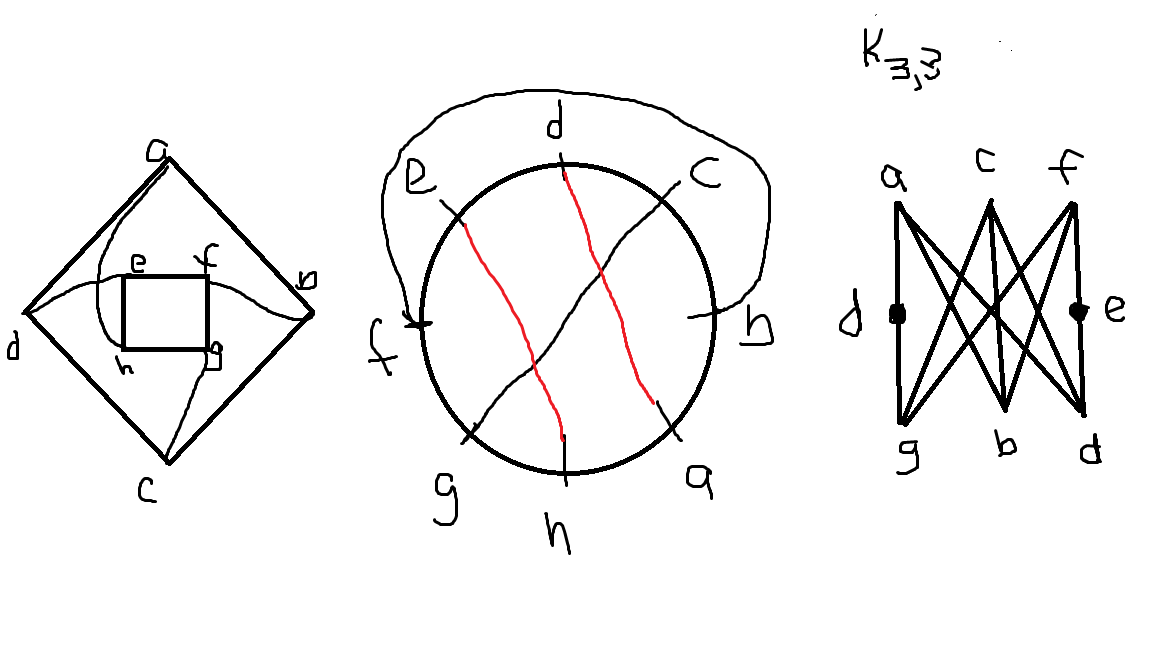
\includegraphics[height=200px]{hw2q3j.png}\newline{}

k. nonplanar - subgraph is a $K_{3,3}$ subdivision\newline{}

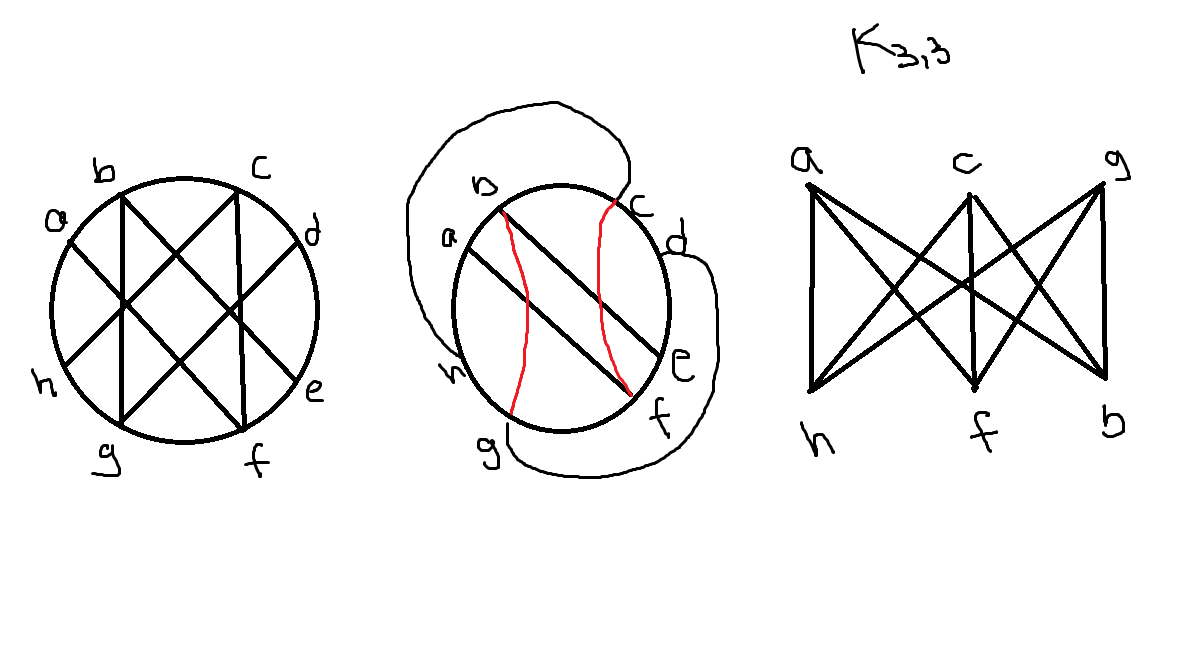
\includegraphics[height=200px]{hw2q3k.png}\newline{}

\underline{Section 1.4 Problem 4}\newline{}

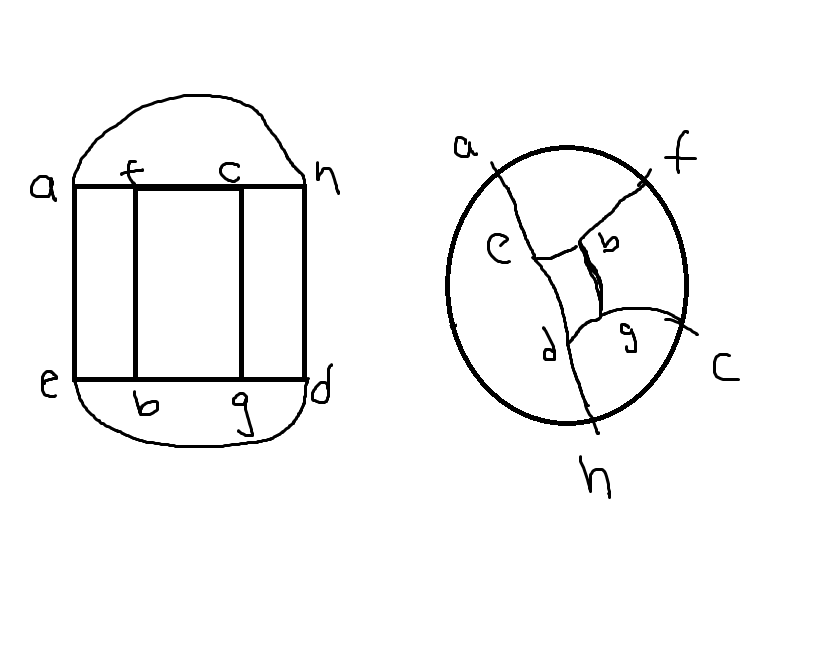
\includegraphics[height=200px]{hw2q4.png}\newline{}

\underline{Section 1.4 Problem 7}\newline{}

e. 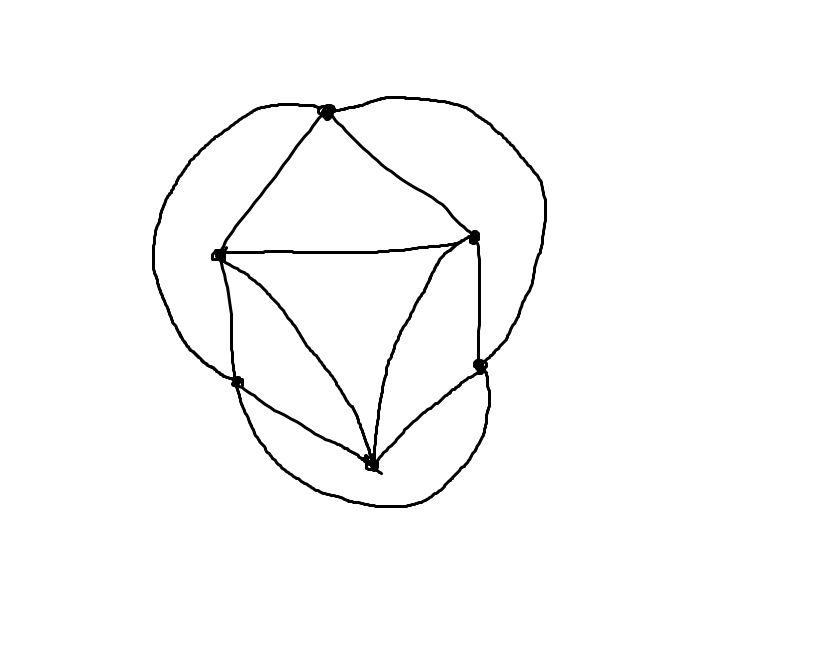
\includegraphics[height=200px]{hw2q7e.png}\newline{}

j. Not possible. If each vertex is of degree 5, this means that the graph is formed of pentagons and that each region is enclosed by 5 edges. The number of edges is equal to the sum of the edges for each region divided by 2. 17 regions * 5 edges each = 85. It is not possible to have $\frac{85}{2}$ edges.
\end{document}
